\chapter{Literature Review}
% HEI <3 Jeg elsker deg 

\section{Quanser's 3 DOF Helicopter}

The helicopter Quanser supplies is a bench top model of a Tandem rotor helicopter, with 3 \acrfull{dof}. Figure \ref{fig:pic_heli}, taken from their website \cite{quanser_heli}, shows a picture of this. 

\begin{figure}[h!]
    \centering
    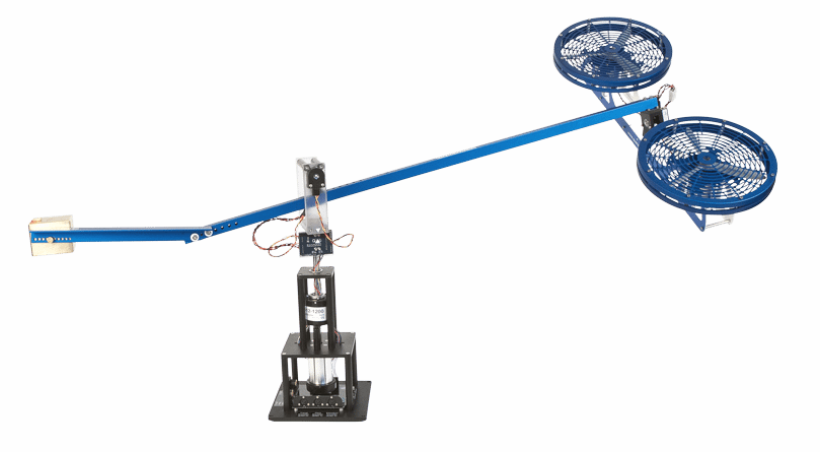
\includegraphics[scale=0.5]{fig/helicopter.png}
    \caption{Picture of Quanser's 3 DOF Helicopter}
    \label{fig:pic_heli}
\end{figure}

In addition, the helicopter comes with a Q8-USB 8 Channel USB Data Acquisition Board and the VoltPAQ-X2 2 Channel Linear Voltage Amplifier, also from Quanser. For Simulink use, it comes with the software package, QUARC.


Since this hardware is designed for testing and developing control laws for systems with similar dynamics, there is a lot of research done on this helicopter.

\cite{veeraboina_2018}: A simplified nonlinear model with LQR, LQR based PID, IO Feedback Linearizing and a Direct Adaptive Fuzzy Controller has been implemented on an Arduino Mega. 

\cite{arican_2018}: State-Dependent Riccati Equation based optimal control for a nonlinear system. Linear control method for nonlinear control is inconsistent. 

\cite{kocagil_2017}: Design methods for nonlinear systems. Review of State Dependent Riccati Equation based optimal control, Model Reference Adaptive Control and Sliding Mode Control. 

\cite{jafri_2017}: Design and apply a fuzzy logic controller. Fuzzy logic controller is a type of control based on fuzzy logic where logical variables take on continuous values between 0 and 1. This is an advantage when dealing with a complex, or "expensive" process model. Compared with a PID, it is concluded that the proposed controller performs better.

\cite{yang_2019}: Multiple helicopters, a fault-tolerant robust adaptive control algorithm is proposed that synchronizes multiple helicopters with actuator faults.

However, none of the existing control suggestion are very equipped for constraint handling. This is the advantage of \acrshort{mpc}. Some \acrshort{mpc}-implementations have been presented.

\cite{Zhai2010}: Nonlinear Model Predictive Control to control elevation and travel using successive linearization to approximate the internal model of the system, and performance is compared to linear \acrshort{mpc}.

Using \acrshort{nmpc} for the helicopter is not feasible given its fast dynamics. Helicopter control is 10 Hz, which is nearly impossible for microcontrollers to run at that speed using \acrlong{nmpc}.

\cite{Tondel2002}: Explicit piecewise linear state feedback solutions to constrained \acrshort{mpc} gives larger offline complexity. Paper studies two approaches to complexity reduction, input trajectory parametrization and search tree that allows PWL function to be implemented in real time. However, this deals with explicit \acrshort{mpc}. 

\cite{ju_2014}: \acrfull{empc} of the helicopter is presented in simulation and semi-physical simulation. Proves feasibility and performance of \acrshort{empc}-algorithm. 

\cite{cheng_2016}: \acrfull{empc} for attitude regulation and tracking, compared with a \acrshort{pid}-controller. 


\acrfull{empc} is a version of \acrshort{mpc} that reduces the online computational cost of the control by moving all those calculations offline. This entails providing an explicit optimal control law  by calculating all possible optimal input trajectories in the operating region of the system. 

This is not feasible because



The closest research to what is presented in this thesis:
\cite{Zhai2013}: An observer based \acrshort{mpc} with successive linearization, which uses the current state of the system to linearize a nonlinear process model about that point and use the linear model in the \acrshort{mpc}, online. This paper focuses on a performance comparison between the use of unscented Kalman filter and other filters, like linear filter and extended Kalman filter. The \acrshort{qp}-problem used in the \acrshort{mpc} is without a terminal constraint or cost.

The work presented in this thesis has a larger focus on the concept of \textit{stable} \acrlong{mpc} - the effects of adding a terminal cost and constraint.



\section{Embedded Optimization}


Embedded optimization is the concept of continuously solving an optimization problem where the data is update real-time from a system the evolves over time. Naturally, the exact evolution of the system can only be predicted to a certain degree, and the optimization should be dynamic, as in a function of time and the process. Embedded optimization is complex, mainly because of the close relationship between the solver, the hardware and the process \cite{embedded_optimization}.

In the late 1970s, \acrlong{mpc} was introduced as a combination of feedback control theory and numerical optimization \cite{mpc_early}, and quickly gained traction as a constraint handling control method, mostly used in the petrochemical and process industry. As the computer was introduced and popularized a few decades later, optimization methods on embedded hardware was introduced to address needs such as cost effectiveness and efficient energy use. Now the technology mostly used in a specific industry could be applied to areas such as robotics, aerospace and automotive. With this development challenges related to algorithms and their implementations, as well as the computing hardware arises. 

The concept of embedded \acrshort{mpc} arises from this development. Thirty years ago, this algorithm was run on computers at low frequencies, as slow as calculations once a minute \cite{qin_badgwell}. 

Over the last thirty years, a lot of \acrshort{mpc} implementations have been introduced, mostly solving the \acrshort{qp}-problem on a computer at a low frequency. However, more recently, solving these optimization problems on embedded hardware has been done for \acrfull{cpu}s, digital signal processors, programmable logic controllers and \acrfull{fpga}s \cite{embedded_optimization_control}.

The topic of embedded \acrshort{mpc} is an increasingly en popular one, as it is being proposed for smaller and smaller systems. \acrshort{mpc} has become an increasingly popular control method, given it can solve problems with physical constraints. The demand for this technology to work in embedded systems is only natural. An obstacle in this is the computational cost, and therefore time requirement. This is where, for example OSQP comes in, a \acrshort{qp}-solver perfectly suited for \acrshort{mpc} in embedded.

A few examples are using MPC for controlling a hovercraft, and a path following MPC for serial-link robot manipulators \cite{embedded_optimization_control}. 


The existing control solutions for embedded systems, \acrshort{pid}-controller, Kalman filter, \acrshort{lqr}, needs a lot of tuning to cope with constraints and nonlinearities. Introduction \acrshort{mpc} removes this problem. However, problems arise when considering the online computational cost of \acrlong{mpc}, therefore this concept warrants extra attention. 


